\subsection{Estimation of roll damping from roll decay tests}
\label{se:experimental_estimation}
In order to extract roll damping parameters from the roll decay tests, parameters in the cubic, quadratic or linear roll decay models should be identified. The roll angle is measured during the roll decay tests. The system identification is defined as finding the parameters that produce a simulated roll signal that best fits the roll decay test measurement. 
To evaluate the performed tests, a modified version of the PIT approach is developed. This modified approach adds a time-dependent second-degree polynomial to the fitting. It later can be separated from the solution to account for low frequency disturbances. The roll equation that is used for the evaluation has a linear-quadratic damping dependence and a linear restoring term. A quadratic roll damping model can be linearized using the equivalent linear damping coefficient \parencite{himeno_prediction_1981}:

\begin{equation}
B_{e} = B_{1} + \frac{8 B_{2} \omega_{0} \phi_{a}}{3 \pi}
\end{equation}


In order to obtain the damping coefficients $B_1$ and $B_2$, roll damping is calculated for two or more roll amplitudes $\phi_a$ for the same motion frequency (for this study, it is referred to the natural frequency $\omeg$ because free roll decay tests were used for the model tests.). $B_1$ and $B_2$ is obtained by fitting equation \ref{eq:B_e_equation} to this data as shown in figure \ref{fig:ikeda_B_1_B2}.  

\begin{figure}[H]
    \centering
    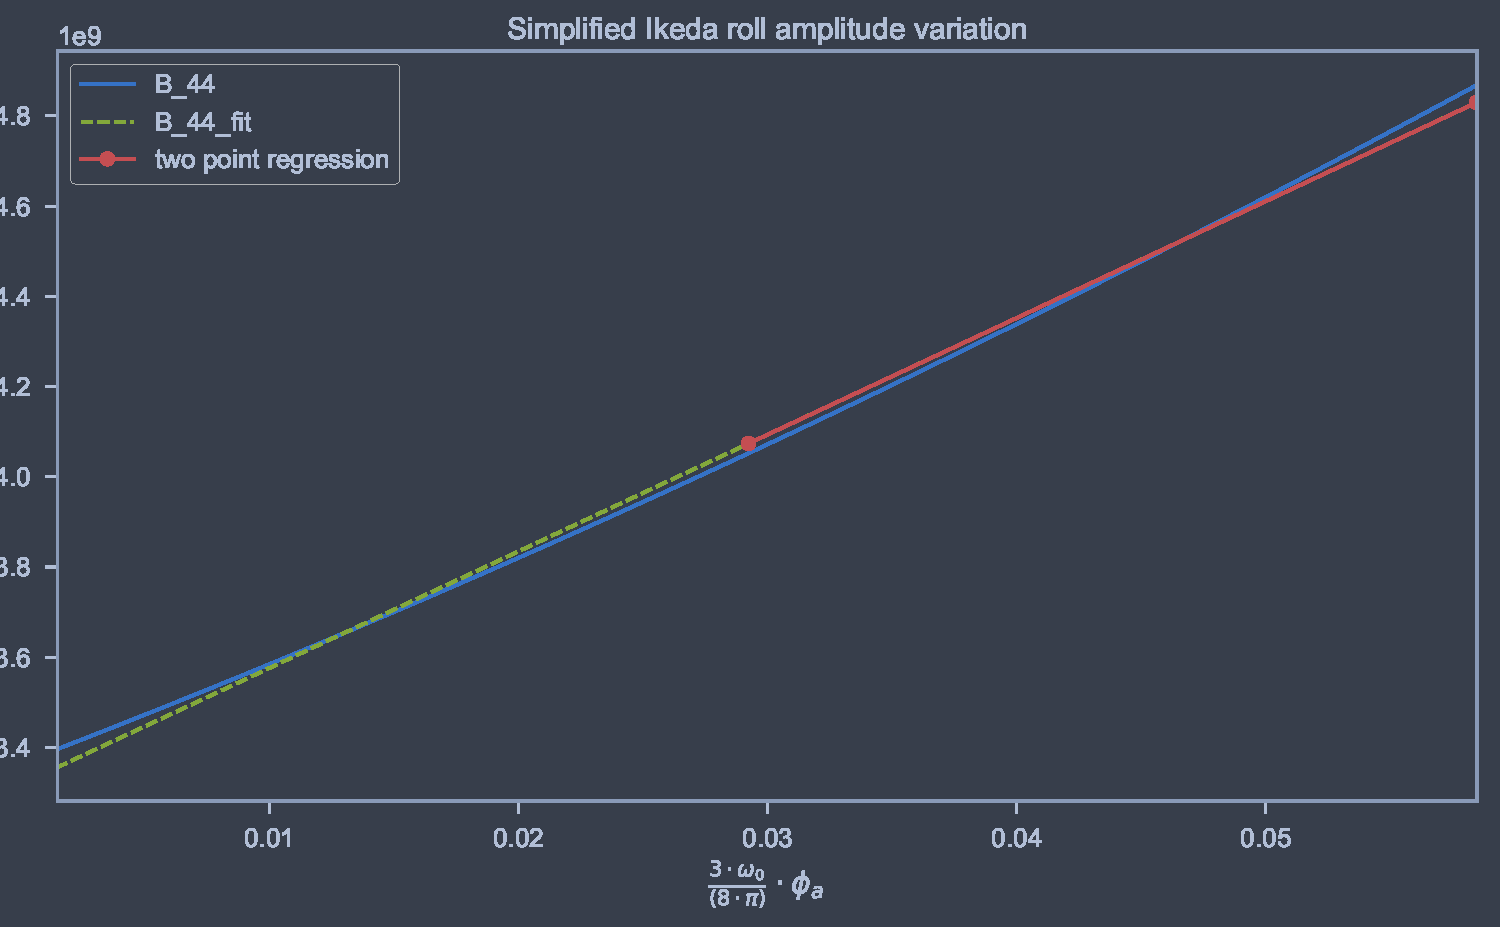
\includegraphics[height=5cm, width=8cm]{figures/ikeda_B_1_B_2.pdf}
    \vspace{-0.5cm}
    \caption{Variation of roll amplitude to derive $B_1$ and $B_2$}
    \label{fig:ikeda_B_1_B2}
\end{figure}




%Peter Piehl \parencite{henry_peter_piehl_ship_nodate} shows an analytical solution %to the linear model in equation \ref{eq:roll_decay_equation_himeno_linear}, %where the natural frequency of the motion is obtained by:
%\begin{equation}
\omega_{0} = \sqrt{\frac{C}{A_{44}}}
\end{equation}

%
%The roll damping and the natural frequency can be made non dimensional using %the following expressions \parencite{himeno_prediction_1981}: 
%\begin{equation} \label{eq:B44_hat_equation}
B_{44 hat} = \frac{\sqrt{2} \sqrt{\frac{beam}{g}} \operatorname{B_{44}}\left(\dot{\phi}\right)}{2 Disp beam^{2} \rho}
\end{equation}

%\begin{equation} \label{eq:omega_hat_equation}
\omega_{hat} = \frac{\sqrt{2} \omega \sqrt{\frac{beam}{g}}}{2}
\end{equation}

%The ordinary differential equations for roll motion in equation \ref{eq:roll_decay_equation_cubic}, \ref{eq:roll_decay_equation_himeno_quadratic} and \ref{eq:roll_decay_equation_himeno_linear} are solved numerically using Explicit Runge-Kutta method of order 5(4). 

%Figure \ref{fig:analytical} shows a comparison for the linear model between this kind of numerical solution and the exact analytical solution \parencite{henry_peter_piehl_ship_nodate}. It seems that the numerical solution agrees well with the analytical. 

%\begin{figure}[h]
%    \centering
%    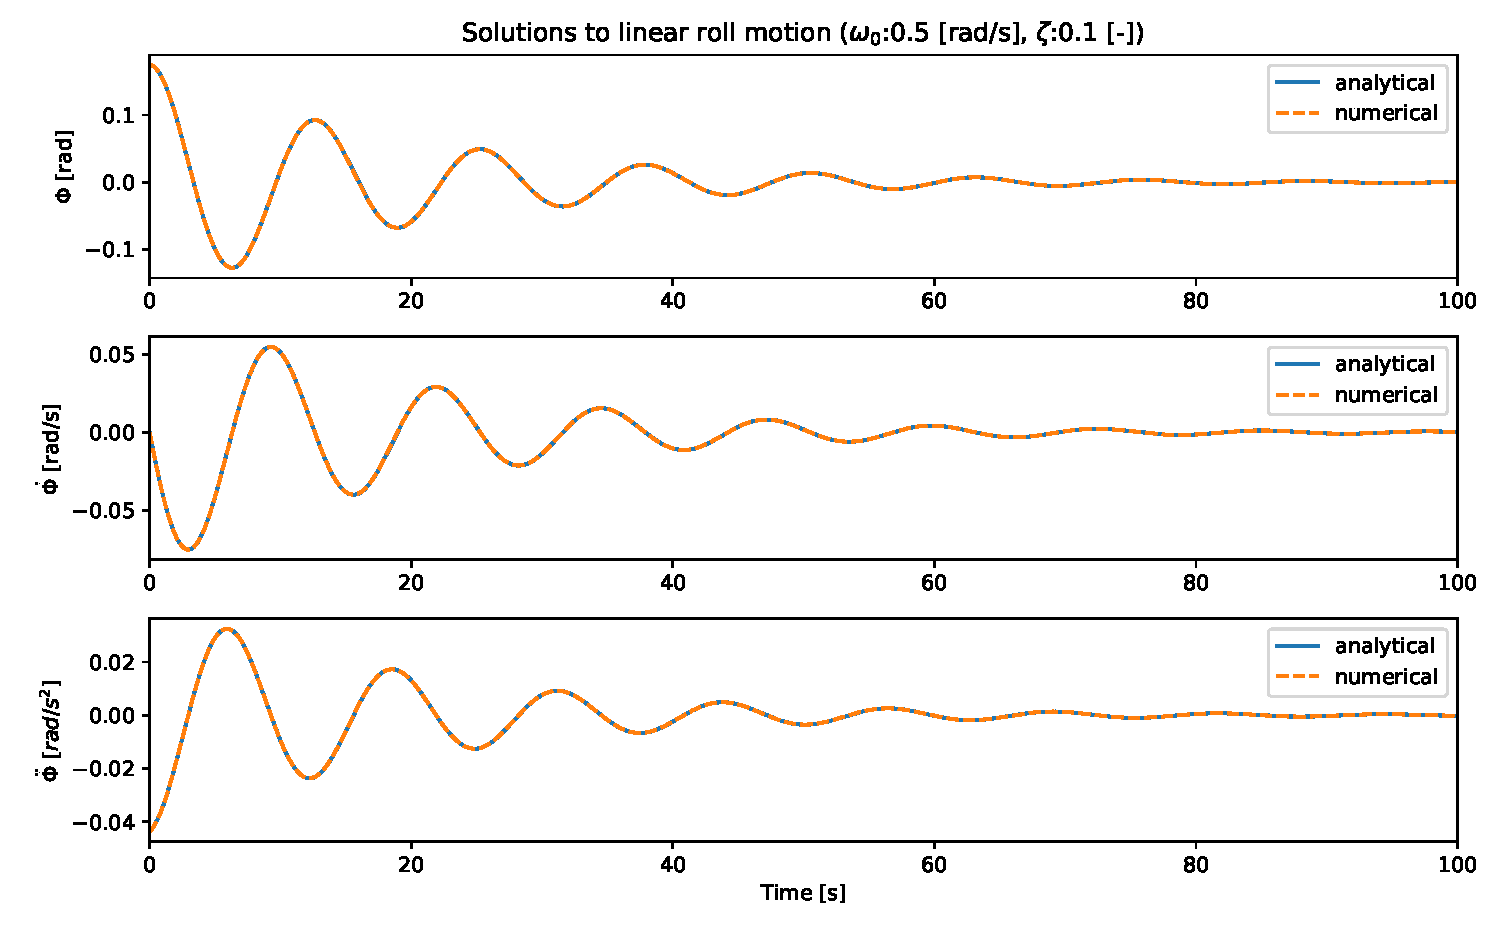
\includegraphics[width=\columnwidth]{figures/analytical.pdf}
%    \caption{Analytical and numerical solution to the linear model}
%    \label{fig:analytical}
%\end{figure}


%\subsection{Parameter Identification Technique}
%\label{se:PIT}
It should be noted that even though the approach could well handle roll equations with higher order of non-linearities in the damping term as well as a non-linear restoring term, the limited amplitudes at which the roll decay tests were conducted cannot motivate advantages of higher order models. 
The goodness of the fit is described using the coefficient of determination:
\begin{equation} \label{eq:R2}
R^2=1-\frac{SS_{res}}{SS_{tot}}
\end{equation}
where $SS_{res}$ is sum of squares of residuals and $SS_{tot}$ is total sum of squares. Two different solution approaches have been investigated for the system identification: a "Derivation approach" and an "Integration approach". 
The "Derivation approach" has the advantage of being very much faster than the "Integration approach" but also the disadvantage of needing to calculate the numerical derivatives which for measurement data also requires some low pass filtration. The "Integration approach" may however also have a disadvantage of not converging.



In the "Derivation approach" the first and second roll time derivatives are calculated numerically so that the parameters in the models are the only unknowns and the optimal parameters that gives the best fit can simply be determined using a least square fit.
In the "Integration approach" the parameters are found by solving a nonlinear least-squares problem using the least-square method \parencite{noauthor_scipyoptimizeleast_squares_nodate} and the Trust Region Reflective algorithm with smooth approximation of l1 (absolute value). This approach requires that ordinary differential equation is solved for many "guessed" sets of parameters till the solution converges.

\begin{figure}[H]
    \centering
    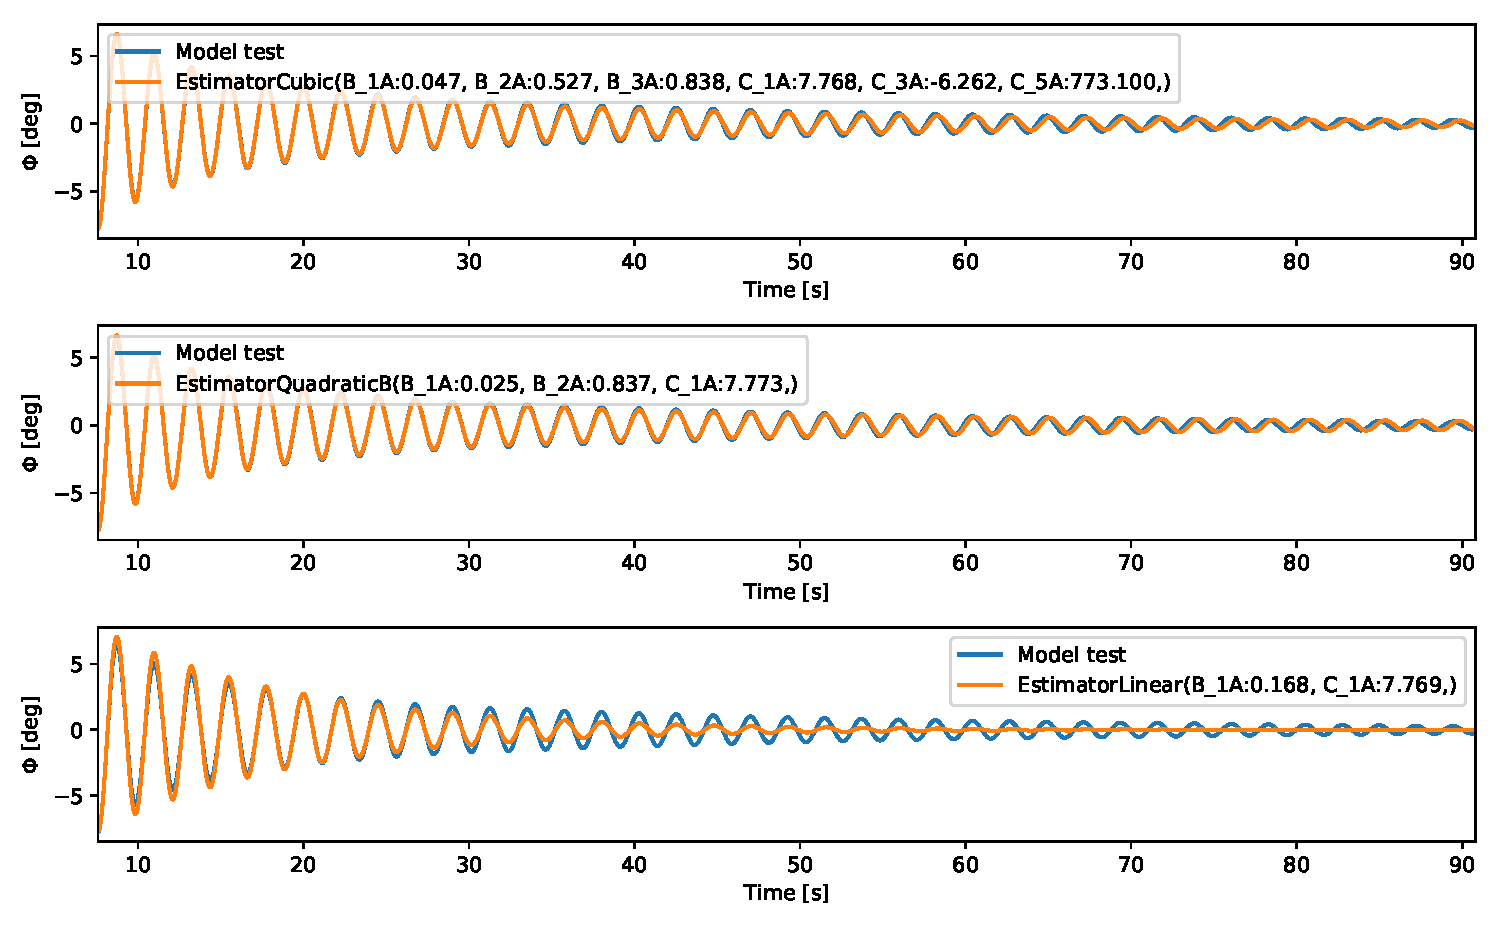
\includegraphics[width=12cm, height = 6cm ]{figures/roll_decay_model_compare.pdf}
    \caption{Roll decay test comparison of linear, quadratic and cubic model}
    \label{fig:roll_decay_model_compare}
\end{figure}

A validation of the developed system identification method has been conducted by checking that known parameters from signals from simulations with the linear, quadratic and cubic models can all be identified. For example,
Figure \ref{fig:roll_decay_model_compare} shows a comparison between the linear, quadratic and cubic model for a random chosen roll decay test motion results. It can be seen that the linear model can not give a perfect representation for the whole range of roll angles.    


